%%%%%%%%%%%%%%%%%%%%%%%%%%%%%%%%%%%%%%%%%%%%%%%%%%%%%%%%%%%%%%%%%%%%%%
% Lớp 10 | Phương pháp tọa độ trong mặt phẳng (𝑂𝑥𝑦) | Đường thẳng trong mặt phẳng tọa độ
% Dạng 0H9?3-2: Phương trình đường thẳng
% Số câu: 58  (sinh tự động bởi tach_cau.py; từ nay thầy sửa trực tiếp file này)
%%%%%%%%%%%%%%%%%%%%%%%%%%%%%%%%%%%%%%%%%%%%%%%%%%%%%%%%%%%%%%%%%%%%%%

%%%%%%%%%%%%%%%% TRẮC NGHIỆM 4 PHƯƠNG ÁN %%%%%%%%%%%%%%%%

% nguồn: MaHoaNH_TracNghiem_Lop10
\begin{ex}%[0H9N3-2]%[ma:7abbeb90]
	Trong mặt phẳng $Oxy$, phương trình tham số của đường thẳng đi qua điểm $M(2;-3)$ và có  véc-tơ chỉ phương $\overrightarrow{u}=(4;1)$ là
	 \choice
		{$\heva{&x=4+2t\\&y=1-3t}$} 
		 {$\heva{&x=-2+4t\\&y=3+t}$}
		 {\True $\heva{&x=2+4t\\&y=-3+t}$}
		 {$\heva{&x=2-3t\\&y=4+t}$}
	\loigiai{Phương trình tham số của đường thẳng đi qua  điểm $M(2;-3)$ và có véc-tơ chỉ phương $\overrightarrow{u}=(4;1)$ là $\heva{&x=2+4t\\&y=-3+t.}$}
\end{ex}

% nguồn: MaHoaNH_TracNghiem_Lop10
\begin{ex}%[0H9N3-2]%[ma:c66578a9]
	Đường thẳng đi qua $A(-1; 2)$, nhận $\overrightarrow{n}=(2;-4)$ làm véctơ pháp tuyến có phương trình  là
	\choice 
		{$x-2y-4=0$} 
		{$x+y+4=0$} 
		 {$-x+2y-4=0$}
		{\True $x-2y+5=0$} 
	\loigiai{Gọi $(d)$ là đường thẳng đi qua $A(-1; 2)$ và nhận $\overrightarrow{n}=(2;-4)$ làm vectơ pháp  tuyến \break
	$\Rightarrow(d)\colon  x+1-2(y-2)=0 \Leftrightarrow x-2y+5=0$.}
\end{ex}

% nguồn: MaHoaNH_TracNghiem_Lop10
\begin{ex}%[0H9N3-2]%[ma:7b28334a]
	Cho đường thẳng  $d\colon-3x+2y-4=0$. Một véc-tơ pháp tuyến của đường thẳng là
	 \choice
		{$\overrightarrow{n}=\left(3;2\right)$} 
		 {$\overrightarrow{n}=\left(-3;-2\right)$}
		{\True $\overrightarrow{n}=\left(-3;2\right)$} 
		{$\overrightarrow{n}=\left(2;3\right)$} 
	\loigiai{Đường thẳng  $d$ nhận $\overrightarrow{n}=(-3;2)$ làm một véc-tơ pháp tuyến.
	 }
\end{ex}

% nguồn: MaHoaNH_TracNghiem_Lop10
\begin{ex}%[0H9N3-2]%[ma:2c098a16]
	Vectơ nào dưới đây  là một vectơ chỉ phương của đường thẳng đi qua hai điểm $A(-3; 2)$ và $B(1; 4)$?
	\choice 
		 {$\vec{u}_1=(-1; 2)$}
		{\True $\vec{u}_2=(2; 1)$} 
		{$\overrightarrow{u_3}=(-2; 6)$} 
		{$\overrightarrow{u_4}=(1;  1)$}
	\loigiai{ 
		Ta có $\overrightarrow{AB}=(4; 2)$ nên một vectơ chỉ phương của  đường thẳng $AB$ cùng phương với $\overrightarrow{AB}=(4; 2)$.\\
	Ta thấy $\vec{u}_2=(2; 1)=\dfrac{1}{2} \overrightarrow{AB}$ suy ra $\vec{u}_2=(2; 1)$ là một vectơ chỉ phương của $AB$.} 
\end{ex}

% nguồn: MaHoaNH_TracNghiem_Lop10
\begin{ex}%[0H9N3-2]%[ma:2e6374de]
	Đường thẳng đi qua điểm $A\left(1;-2\right)$  và nhận $\overrightarrow{n}=\left(-2;4\right)$ làm vectơ pháp tuyến có phương trình
	 \choice
		 {$x+2 y+4=0$}
		{$x-2 y+4=0$} 
		{\True  $x-2 y-5=0$}
		{$-2  x+4 y=0$}
	\loigiai{ 
		Đường  thẳng đi qua điểm $A\left(1;-2\right)$ và nhận $\overrightarrow{n}=\left(-2;4\right)$ làm vectơ pháp tuyến có phương trình là $-2\left(x-1\right)+4\left(y+2\right)=0$ $\Leftrightarrow-2x+4y+10=0$ $\Leftrightarrow x-2y-5=0$.
	 }
\end{ex}

% nguồn: MaHoaNH_TracNghiem_Lop10
\begin{ex}%[0H9N3-2]%[ma:861e9226]
	Phương trình tổng quát của đường thẳng đi qua $A\left(1;\;-2\right)$ và nhận $\overrightarrow{n}=\left(-1;\; 2\right)$ làm vectơ pháp tuyến có  phương trình là
	 \choice
		 {$-x+2y=0$}
		 {$x+2y+4=0$}
		{\True  $x-2y-5=0$}
		{$x-2y+4=0$} 
	 \loigiai{
		Phương trình  đường thẳng là $-1\left(x-1\right)+2\left(y+2\right)=0$ hay $x-2y-5=0$.
	 }
\end{ex}

% nguồn: MaHoaNH_TracNghiem_Lop10
\begin{ex}%[0H9N3-2]%[ma:ecbc9cc4]
	Trong mặt phẳng $Oxy$, cho hai điểm $A(3;-1)$ và  $B(-2;1)$. Viết phương trình đường thẳng $AB$.
	 \choice
		 {\True $2x+5y-1=0$}
		{$5x+2y+1=0$} 
		{$2x-5y+11=0$} 
		 {$5x-2y+11=0$}
	\loigiai{Ta có $\overrightarrow{AB}=(-5;2)$, khi đó đường thẳng $AB$ nhận vectơ $\vec{n}=(2;5)$ làm vectơ pháp tuyến.\\ 
		Phương trình đường  thẳng $AB$ có dạng:
	$2(x-3)+5(y+1)=0 \Leftrightarrow 2x-6+5y+5=0 \Leftrightarrow 2x+5y-1=0$.} 
\end{ex}

% nguồn: MaHoaNH_TracNghiem_Lop10
\begin{ex}%[0H9N3-2]%[ma:845dc651]
	Trong mặt phẳng toạ độ $Oxy$, một véc-tơ chỉ phương của đường thẳng $ d \colon \heva{&x=2+4t \\ &y=3-t}$ có tọa  độ là
	\choice 
		 {\True $(4;-1)$}
		 {$(3;2)$}
		{$(2;3)$} 
		 {$(4;1)$}
	\loigiai{ 
		Đường thẳng $ d \colon \heva{&x=2+4t \\  &y=3-t}$ có một véc-tơ chỉ phương có tọa độ là $(4;-1)$.
	 }
\end{ex}

% nguồn: MaHoaNH_TracNghiem_Lop10
\begin{ex}%[0H9N3-2]%[ma:efb676c9]
	Phương  trình nào sau đây là phương trình tổng quát của một đường thẳng?
	 \choice
		{$y^2=4x$} 
		{$\heva{&x=4+3t\\&y=2-t}$} 
		 {$\dfrac{x^2}{25}+\dfrac{y^2}{9}=1$}
		{\True $4x-3y-2=0$} 
	 \loigiai{
		Phương trình tổng quát của một  đường thẳng là $4x-3y-2=0$.
	 }
\end{ex}

% nguồn: MaHoaNH_TracNghiem_Lop10
\begin{ex}%[0H9N3-2]%[ma:e8797330]
	Trong mặt phẳng tọa độ $Oxy$, đường thẳng $d\colon\heva{&x=1+2t\\&y=2-t}$ đi qua điểm  nào sau đây?
	\choice 
		 {$A(-1;1)$}
		{$B(5;2)$} 
		{$C(3;1)$} 
		 {$D(7;5)$}
	 \loigiai{
		Thay lần lượt tọa độ các điểm $A$,  $B$, $C$, $D$ vào phương trình của $d$ ta thấy chỉ có điểm $C(3;1)$ thỏa mãn.\\
	Vậy đường thẳng $d$ đi qua điểm  $C(3;1)$.}
\end{ex}

% nguồn: MaHoaNH_TracNghiem_Lop10
\begin{ex}%[0H9N3-2]%[ma:2927f8d9]
	Trong mặt phẳng $Oxy$, đường thẳng đi qua hai  điểm $A(3;-7)$ và $B(1;-7)$ có phương trình là
	 \choice
		 {$x+y+6=0$}
		{$x+y+4=0$} 
		{\True $y+7=0$} 
		 {$y-7=0$}
	 \loigiai{ Véc-tơ chỉ phương của đường thẳng $AB$ là $\overrightarrow{u}=\overrightarrow{AB}=(-2;0)$. Suy ra véc-tơ pháp tuyến của đường thẳng $AB$ là $\overrightarrow{n}=(0;2)$. \\
		Phương  trình đường thẳng $AB$ đi qua điểm $A(3;-7)$ và có véc-tơ pháp tuyến $\overrightarrow{n}=(0;2)$ là
		 \[0(x-3)+2(y+7)=0\Leftrightarrow y+7=0.\]
	 }
\end{ex}

% nguồn: MaHoaNH_TracNghiem_Lop10
\begin{ex}%[0H9N3-2]%[ma:9b58e4a9]
	Phương trình tham số  của đường thẳng qua $M\left(1;-1\right)$, $N\left(4;3\right)$ là
	\def\dotEX{} 
	 \choice
		{$\heva{&{x=3+t} \\  &{y=4-t}.}$}
		 {$\heva{&{x=1+3t} \\&{y=1+4t}.}$}
		{$\heva{&{x=3-3t} \\&{y=4-3t}.}$} 
		 {\True $\heva{&{x=1+3t} \\&{y=-1+4t}.}$}
	\loigiai{ 
		Đường thẳng đi qua hai điểm $M\left(1;-1\right)$, $N\left(4;3\right)$ có một vectơ chỉ phương  $\overrightarrow{MN}=\left(3;\; 4\right)$.\\
		Phương  trình tham số của đường thẳng qua $M\left(1;-1\right)$, $N\left(4;3\right)$ là $\heva{&{x=1+3t} \\&{y=-1+4t}.}$
	 }
\end{ex}

% nguồn: MaHoaNH_TracNghiem_Lop10
\begin{ex}%[0H9N3-2]%[ma:2638a766]
	Viết phương trình tham số của đường thẳng đi qua $A\left(3;4\right)$ và có vectơ chỉ phương  $\overrightarrow{u}=\left(3;-2\right)$
	 \def\dotEX{}
	\choice 
		 {$\heva{&{x=3+3t} \\&{y=-2+4t}.}$}
		 {$\heva{&{x=3-6t} \\&{y=-2+4t}.}$}
		 {$\heva{&{x=3+2t} \\&{y=4+3t}.}$}
		{\True  $\heva{&{x=3+3t} \\&{y=4-2t}.}$}
	 \loigiai{
		Phương trình tham số của đường thẳng đi qua  $A\left(3;4\right)$ và có vectơ chỉ phương $\overrightarrow{u}=\left(3;-2\right)$
		có dạng $\heva{&{x=3+3t}  \\&{y=4-2t}.}$
	} 
\end{ex}

% nguồn: MaHoaNH_TracNghiem_Lop10
\begin{ex}%[0H9N3-2]%[ma:41c5e7c2]
	Đường thẳng $d$ qua $A(1; 1)$ và có véctơ  chỉ phương $\overrightarrow{u}=(2; 3)$ có phương trình tham số là
	 \def\dotEX{}
	\choice 
		{$\heva{&x=1-t \\ &y=3-t.}$} 
		{\True  $\heva{&x=1+2t \\&y=1+3t.}$}
		 {$\heva{&x=2+t \\&y=3+t.}$}
		 {$\heva{&x=2t \\&y=3t.}$}
	\loigiai{ 
		Đường thẳng $d$ qua $A(1; 1)$ và có vectơ chỉ phương $\overrightarrow{u}=(2; 3)$ có phương trình tham  số là
		$$\heva{&x=1+2t \\&y=1+3t.} 
		$$ 
	 }
\end{ex}

% nguồn: MaHoaNH_TracNghiem_Lop10
\begin{ex}%[0H9H3-2]%[ma:db8f286f]
	Cho tam giác $ABC$ có $A(-1;-2)$; $B(0; 2)$; $C(-2; 1)$. Đường trung tuyến $BM$  có phương trình là
	 \choice
		{\True  $5x-3y+6=0$}
		 {$3x-5y+10=0$}
		{$x-3y+6=0$} 
		 {$3x-y-2=0$}
	\loigiai{Gọi $M$ là trung điểm  $AC \Rightarrow M\left(-\dfrac{3}{2};-\dfrac{1}{2}\right)$.\\ Ta có $\overrightarrow{B M}=\left(-\dfrac{3}{2};-\dfrac{5}{2}\right)$.\\
		Đường thẳng $BM$ qua $B(0; 2)$ và nhận $\overrightarrow{n}=(5;-3)$ làm  vectơ pháp tuyến.\\
	 Suy ra $BM\colon 5x-3(y-2)=0 \Leftrightarrow 5 x-3y+6=0$.}
\end{ex}

% nguồn: MaHoaNH_TracNghiem_Lop10
\begin{ex}%[0H9H3-2]%[ma:ba2674a7]
	Viết phương trình đường thẳng đi qua điểm $A(3;2)$ và nhận $\vec{n}=(2;-4)$ làm vectơ pháp  tuyến.
	 \choice
		{\True $x-2y+1=0$} 
		 {$x-2y-7=0$}
		 {$3x-2y+4=0$}
		{$2x+y-8=0$} 
	\loigiai{ 
		Ta có phương trình dạng  $2(x-3)-4(y-2)=0 \Leftrightarrow x-2y+1=0$.
	 }
\end{ex}

% nguồn: MaHoaNH_TracNghiem_Lop10
\begin{ex}%[0H9H3-2]%[ma:26141896]
	Phương trình tham số của đường  thẳng qua $A(1;-2)$, $B(4;3)$ là
	\choice 
		{$\heva{&x=4+t\\&y=3-2t}$} 
		 {$\heva{&x=3+3t\\&y=4+5t}$}
		{$\heva{&x=1+5t\\&y=-2-3t}$} 
		{\True  $\heva{&x=1+3t\\&y=-2+5t}$}
	\loigiai{Ta có  $\overrightarrow{AB}=(3;5)$.\\
		Phương trình tham số của đường thẳng qua $A(1;-2)$, $B(4;3)$ có  véc-tơ chỉ phương là $\overrightarrow{AB}=(3;5)$ có phương trình $\heva{&x=1+3t\\&y=-2+5t.}$
	} 
\end{ex}

% nguồn: MaHoaNH_TracNghiem_Lop10
\begin{ex}%[0H9H3-2]%[ma:cb7fda30]
	Trong mặt phẳng $Oxy$, phương trình đường thẳng đi qua  hai điểm $A(-2;4)$, $B(-6;1)$ là
	 \choice
		 {$3x+4y-10=0$}
		 {\True $3x-4y+22=0$}
		 {$3x-4y+8=0$}
		 {$3x-4y-22=0$}
	 \loigiai{
		Phương trình đường thẳng đi qua hai  điểm $A(-2;4)$, $B(-6;1)$ có dạng $$AB\colon\dfrac{x+2}{-4}=\dfrac{y-4}{-3}\Rightarrow 3x-4y+22=0.$$
	Vậy đường thẳng đi qua $A$ và $B$ có  phương trình $3x-4y+22=0$.}
\end{ex}

% nguồn: MaHoaNH_TracNghiem_Lop10
\begin{ex}%[0H9H3-2]%[ma:1c1ec6b2]
	Trên mặt phẳng tọa độ $Oxy$, phương trình tham số của đường thẳng đi  qua hai điểm $A(3;-1)$, $B(1;3)$ là
	\choice 
		 {$\heva{&x=-2+3t\\&y=4-t}$}
		 {$\heva{&x=1+2t\\&y=3+t}$}
		 {\True $\heva{&x=1-2t\\&y=3+4t}$}
		 {$\heva{&x=1-2t\\&y=3+2t}$}
	 \loigiai{
		Ta  có $\overrightarrow{AB}=(-2;4)$ là véc-tơ chỉ phương của đường thẳng và qua $B(1;3)$ có phương trình tham số là $\heva{&x=1-2t\\&y=3+4t.}$
	} 
\end{ex}

% nguồn: MaHoaNH_TracNghiem_Lop10
\begin{ex}%[0H9H3-2]%[ma:4b5af18d]
	Đường thẳng  đi qua hai điểm $M(-1; 2)$, $N(3; 1)$ có phương trình tổng quát là
	 \choice
		 {$4x-y-6=0$}
		{$2x+3y-9=0$} 
		{$x-4y+9=0$} 
		{\True  $x+4y-7=0$}
	 \loigiai{
		 Ta có $\overrightarrow{MN}=(4;-1)$ là vectơ chỉ phương của đường thẳng $MN$ do đó $\overrightarrow{n}=(1; 4)$ là một vectơ pháp tuyến của đường thẳng $MN$.\\
		Phương trình tổng quát của  đường thẳng $MN$ là $1(x+1)+4(y-2)=0 \Leftrightarrow x+4y-7=0$.
	 }
\end{ex}

% nguồn: MaHoaNH_TracNghiem_Lop10
\begin{ex}%[0H9H3-2]%[ma:51b42f45]
	Trên mặt phẳng tọa độ $Oxy$, phương trình của  đường thẳng $d$ đi qua điểm $A(2;-1)$ có véc-tơ pháp tuyến $\overrightarrow{n}=(3;2)$ là
	\choice 
		{\True $3x+2y-4=0$} 
		{$3x+2y+4=0$} 
		 {$2x-3y-7=0$}
		{$3x-2y-8=0$} 
	\loigiai{ 
		Phương trình của đường thẳng $d$ đi qua điểm $A(2;-1)$ có véc-tơ pháp tuyến  $\overrightarrow{n}=(3;2)$ là
		 $$3(x-2)+2(x+1)=0\Leftrightarrow 3x+2y-4=0.$$
	} 
\end{ex}

% nguồn: MaHoaNH_TracNghiem_Lop10
\begin{ex}%[0H9H3-2]%[ma:61a8f290]
	Trong mặt phẳng $Oxy$, cho tam giác $ABC$ có  $A(2;-1)$, $B(4;5)$ và $C(-3;2)$. Phương trình tổng quát của đường cao kẻ từ đỉnh $A$ của tam giác $ABC$ là
	\choice 
		{\True  $7x+3y-11=0$}
		 {$3x+7y+1=0$}
		{$7x+3y+11=0$} 
		 {$-7x+3y+11=0$}
	\loigiai{ 
		Do $AH\perp BC$  nên $AH$ nhận $\overrightarrow{BC}=(-7;-3)$ làm véc-tơ pháp tuyến.\\
		$AH$ đi  qua $A$ nên ta có phương trình $-7(x-2)-3(y+1)=0\Leftrightarrow 7x+3y-11=0$.
	} 
\end{ex}

% nguồn: MaHoaNH_TracNghiem_Lop10
\begin{ex}%[0H9H3-2]%[ma:14a12c9b]
	Trong mặt phẳng toạ độ $Oxy$,  cho hai điểm $A\left( 4;-1 \right)$ và $B\left(2;3 \right)$, phương trình tham số của đường thẳng $AB$ là
	\choice 
		{$\heva{&  x=4+t \\& y=1-2t}$}
		{$\heva{& x=4+t  \\& y=3-2t}$}
		{\True $\heva{& x=2-t \\& y=3+2t}$} 
		{$\heva{& x=2+t \\&  y=-3+2t}$}
	 \loigiai{
		Đường thẳng $AB$ có  một véc-tơ chỉ phương là $\overrightarrow{u}=\dfrac{1}{2}\overrightarrow{AB}=(-1;2)$.\\
		Phương trình đường thẳng  $AB$ là $\heva{& x=2-t \\& y=3+2t.}$
	 }
\end{ex}

% nguồn: MaHoaNH_TracNghiem_Lop10
\begin{ex}%[0H9H3-2]%[ma:ca8ec38c]
	Trong mặt phẳng toạ độ $Oxy$, phương trình tổng quát  của đường thẳng đi qua $A(3;-2)$, $B(4;-1)$ là
	\choice 
		 {$x-y-1=0$}
		 {$x-y-5=0$}
		{$x+y+5=0$} 
		{\True $x+y-1=0$} 
	\loigiai{ 
		Ta có $\overrightarrow{AB}=(1;1)$ suy ra $\overrightarrow{n}=(1;-1)$ là véc-tơ pháp tuyến của đường thẳng  đi qua $A$, $B$.\\
		Vậy phương trình tổng quát của đường  thẳng qua $AB$ là $$(x-3)+(y+2)=0 \Leftrightarrow x+y-1=0.$$
	} 
\end{ex}

% nguồn: MaHoaNH_TracNghiem_Lop10
\begin{ex}%[0H9H3-2]%[ma:1de8f1d3]
	Cho đường thẳng $d\colon 8x-6y+7=0$. Nếu đường thẳng $\Delta$ đi qua gốc tọa độ  và vuông góc với đường thẳng $d$ thì $\Delta$ có phương trình là
	\choice 
		{$4x-3y=0$} 
		{$4x+3y=0$} 
		{\True $3x+4y=0$} 
		 {$3x-4y=0$}
	\loigiai{ 
		Vì $\Delta$ vuông góc với đường thẳng $d\colon 8x-6y+7=0$ nên phương trình 
		$\Delta\colon 6x+8y+C=0$.\\ 
		Mà $\Delta$ đi qua gốc tọa độ  nên ta có $6\cdot 0+8\cdot0+C=0\Leftrightarrow C=0$.\\
	Vậy phương trình  $\Delta\colon 6x+8y=0$ hay $\Delta\colon 3x+4y=0$.}
\end{ex}

% nguồn: MaHoaNH_TracNghiem_Lop10
\begin{ex}%[0H9H3-2]%[ma:6920f598]
	Trong mặt  phẳng $Oxy$, đường thẳng qua điểm $M(4;5)$ và nhận $\vec{u}=(2;3)$ làm véc-tơ chỉ phương có phương trình tham số là
	 \choice
		 {$\heva{&x=2+4t\\&y=3+5t} (t \in \mathbb{R})$}
		{\True $\heva{&x=4+2t\\&y=5+3t} (t \in \mathbb{R})$} 
		{$\heva{&x=4+5t\\&y=2+3t} (t \in \mathbb{R})$} 
		{$\heva{&x=2+t\\&y=5+3t} (t \in \mathbb{R})$} 
	\loigiai{ 
		Đường thẳng qua điểm $M(4;5)$ và nhận $\vec{u}=(2;3)$ làm véc-tơ chỉ phương có phương trình tham số là \begin{center}
		$\heva{&x=4+2t\\&y=5+3t.} (t \in \mathbb{R})$ 
	\end{center}
 }
\end{ex}

% nguồn: MaHoaNH_TracNghiem_Lop10
\begin{ex}%[0H9H3-2]%[ma:74bf7e31]
	Trên mặt phẳng tọa độ $Oxy$, cho hai điểm $A(-2; 3)$ và $B(4;-1)$. Phương trình nào sau đây  là phương trình đường thẳng $AB$?
	\choice 
		 {$x+y-3=0$}
		{$y=2x+1$} 
		 {$\dfrac{x-4}{6}=\dfrac{y-1}{-4}$}
		{\True $\heva{&x=1+3t \\ 
		&y=1-2t}$} 
	 \loigiai{
		Ta có  $\overrightarrow{AB}=(6;-4)$. Khi đó đường thẳng $AB$ có một vectơ chỉ phương là $\overrightarrow{u}=(3;-2)$.\\
		 Trung điểm của đoạn thẳng $AB$ là $I(1;1)$.\\
		Khi đó đường thẳng $AB$ đi qua $I(1;1)$ và có vectơ chỉ  phương $\overrightarrow{u}=(3;-2)$ nên có phương trình $\heva{&x=1+3t \\
		 &y=1-2t.}$
	 }
\end{ex}

% nguồn: MaHoaNH_TracNghiem_Lop10
\begin{ex}%[0H9H3-2]%[ma:c4299245]
	Trong mặt phẳng $ Oxy $ cho điểm $ M(2;1) $.  Gọi $ A, B $ là hình chiếu của $ M $ lên $ Ox, Oy $.
	Phương trình đường  thẳng $ AB $ là
	 \choice
		{$ x + y - 3  = 0 $}
		{$ 2x + y  + 2 = 0 $}
		 {$ 2x + y - 2 = 0 $}
		{\True $ x + 2y -  2 = 0 $}
	\loigiai{ 
		\begin{itemize}
			\item Hình chiếu $ A $ của $  M(2;1) $ lên $ Ox $ là $ A(2;0) $.
			\item Hình chiếu $ B $ của $ M(2;1) $ lên $ Oy  $ là $ B(0;1) $.
		\end{itemize}
		Phương  trình đường thẳng $ AB $ là $x + 2y - 2 = 0.$
	 }
\end{ex}

% nguồn: MaHoaNH_TracNghiem_Lop10
\begin{ex}%[0H9V3-2]%[ma:a04a0005]
	Trong  mặt phẳng $Oxy$, cho tam giác $ABC$ có $A(2;-1)$, $B(4;5)$, $C(-3; 2)$. Phương trình tổng quát của đường cao xuất phát từ đỉnh $A$ là
	\choice 
		 {$3x+7y+1=0$}
		{$-7x+3y+11=0$} 
		{$7x+3y+11=0$} 
		{\True  $7x+3y-11=0$}
	 \loigiai{
		Đường cao xuất phát từ đỉnh $A$ đi qua $A(2;-1)$ và nhận véc-tơ $\overrightarrow{BC}=(-7;-3)$ làm véc-tơ  pháp tuyến nên có phương trình
		$$-7(x-2)-3(y+1)=0\Leftrightarrow -7x-3y+11=0\Leftrightarrow 7x+3y-11=0.$$ 
	} 
\end{ex}

% nguồn: MaHoaNH_TracNghiem_Lop10
\begin{ex}%[0H9Y3-2]%[ma:f6c86894]
	Phương trình  của đường thẳng $\Delta$ đi qua điểm $M(5;4)$ và có véc-tơ pháp tuyến $\overrightarrow{n}=(11;-12)$ là
	 \choice
		 {$5x+4y+7=0$}
		 {$5x+4y-7=0$}
		 {\True $11x-12y-7=0$}
		 {$11x-12y+7=0$}
	\loigiai{ 
		Phương trình tổng  quát của đường thẳng $\Delta$ đi qua điểm $M(5;4)$ và có véc-tơ pháp tuyến $\overrightarrow{n}=(11;-12)$ là
		 $$11(x-5)-12(y-4)=0\Rightarrow 11x-55-12y+48=0\Rightarrow 11x-12y-7=0.$$
	 }
\end{ex}


%%%%%%%%%%%%%%%% ĐÚNG/SAI %%%%%%%%%%%%%%%%

% nguồn: MaHoaNH_DungSai_Lop10
\begin{ex}%[0H9N3-2]%[ma:1b2fce7f]
	Các mệnh đề sau đúng hay sai? 
	\choiceTF 
		{\True $\Delta$ qua điểm $A(-2;1)$ và có vectơ pháp tuyến $\overrightarrow{n}=(3;5)$, khi đó phương trình tổng quát của $\Delta$ là $3x+5y+1=0$} 
		{\True $\Delta$ qua điểm $M(4;3)$ và có vectơ chỉ phương  $\overrightarrow{u}=(6;1)$, khi đó phương trình tổng quát của $\Delta$ là $-x+6y-14=0$}
		{\True $\Delta$ qua  điểm $H(2;-2)$ và $K(-5;-1)$, khi đó phương trình tổng quát của $\Delta$ là $x+7y+12=0$}
		{\True $\Delta$ qua $M(-2,-3)$ và $\Delta \parallel Oy$, khi đó phương trình tổng quát của $\Delta$  là $x+2=0$}
	\loigiai{ 
		\begin{itemchoice}
			\itemch $\Delta$ qua $A(-2;1)$ và vectơ pháp tuyến  $\overrightarrow{n}=(3;5)$.
			\[\Rightarrow \Delta\colon 3(x+2)+5(y-1)=0\Leftrightarrow  \Delta:3x+5y+1=0.\]
			\itemch Vì $\Delta$ có vectơ chỉ phương $\overrightarrow{u}=(6;1)$ nên vectơ  pháp tuyến của $\Delta$ là $\overrightarrow{n}=(-1;6)$.\\
			$\Delta$  qua $M(4;3)$ và vectơ pháp tuyến $\overrightarrow{n}=(-1;6)$.
			\[\Rightarrow  \Delta\colon -1(x-4)+6(y-3)=0\Leftrightarrow \Delta:-x+6y-14=0.
			 \]
			\itemch Vì $\Delta$ có vectơ chỉ phương $\overrightarrow{HK}=(-7;1)$ nên vectơ pháp tuyến của $\Delta$  là $\overrightarrow{n}=(1;7)$.\\ $\Delta$ qua $H(2;-2)$ và vectơ pháp tuyến $\overrightarrow{n}=(1;7)$.
			\[\Rightarrow \Delta\colon 1(x-2)+7(y+2)=0\Leftrightarrow \Delta\colon x+7y+12=0.\] 
			\itemch Qua $M(-2,-3)$ và $\Delta \parallel  Oy$
			$M(-2,-3)\in \Delta$.\\ Vì $\Delta \parallel Oy\Rightarrow$ vectơ pháp tuyến  của $\Delta$ là $\overrightarrow{n_{\Delta}}=\overrightarrow{i}=(1,0)$.\\
			Phương trình tổng quát của  $\Delta\colon 1(x+2)+0(y+3)=0\Leftrightarrow x+2=0$.
		\end{itemchoice}
	 }
\end{ex}

% nguồn: MaHoaNH_DungSai_Lop10
\begin{ex}%[0H9H3-2]%[ma:a703c3d2]
	Trong mặt phẳng với hệ trục tọa độ $Oxy$, cho hai điểm $A(3;-2)$ và $B(1,2)$. Gọi $d$ là đường trung  trực của đoạn thẳng $AB$.
	\choiceTF 
		{\True Tọa độ trung điểm  $I$ của đoạn thẳng $AB$ là $(2;0)$}
		{Một véc-tơ pháp tuyến của đường  thẳng $d$ có tọa độ là $(2;4)$}
		{\True Một véc-tơ chỉ phương của đường thẳng $d$ có tọa độ  là $(2;1)$}
		{Phương trình tham số của  $d$ là $\heva{&x=2+2t \\ &y=1}$ ($t\in\mathbb{R}$)}
	\loigiai{ 
		\begin{itemchoice}
			\itemch Đúng. Trung điểm $I$ của đoạn thẳng $AB$ có tọa độ là $\left( \dfrac{3+1}{2}; \dfrac{-2+2}{2} \right) =  (2;0)$.
			\itemch Sai. Ta có $\overrightarrow{AB}=(-2;4)$ là một véc-tơ pháp tuyến của đường thẳng $d$. Véc-tơ có tọa độ $(2;4)$ không cùng  phương với $\overrightarrow{AB}$ nên không phải là một véc-tơ pháp tuyến của đường thẳng $d$.
			\itemch Đúng. Đường thẳng $d$  có một véc-tơ pháp tuyến là $\overrightarrow{AB} = (-2;4)$, suy ra có một véc-tơ chỉ phương là $\overrightarrow{u} = (2;1)$.
			\itemch Sai. Do đường thẳng $d$ có véc-tơ chỉ phương là $\overrightarrow{u}=(2;1)$ và đi qua điểm $I(2;0)$, nên $d$ có phương trình tham số là  $\heva{&x=2+2t \\ &y=t}$ ($t\in\mathbb{R}$).
		\end{itemchoice}
	 }
\end{ex}

% nguồn: MaHoaNH_DungSai_Lop10
\begin{ex}%[0H9H3-2]%[ma:bca82018]
	Trong mặt phẳng toạ độ  $Oxy$, cho hai điểm $A(-2;2)$, $B(3;4)$. Xét tính Đúng - Sai của các khẳng định sau.
	\choiceTF 
		{Đường thẳng $AB$ có một véc-tơ chỉ phương là $\overrightarrow{AB}=(2;5)$} 
		 {\True Đường thẳng $AB$ có một véc-tơ pháp tuyến là $\vec{n}=(2;-5)$}
		{\True Phương  trình tổng quát của đường thẳng $AB$ là $2x-5y+14=0$}
		{Phương trình tham số của đường thẳng đi qua $M(-1;1)$  và song song với $AB$ là $\heva{&x=-1+2t \\&y=1+5t}$ $(t\in\mathbb{R})$}
	 \loigiai{
		\begin{itemchoice}
			\itemch Đường thẳng $AB$ có véc-tơ chỉ  phương là $\overrightarrow{AB} =(5;2)$.
			\itemch  Đường thẳng $AB$ có véc-tơ chỉ phương là $\overrightarrow{AB}=(5;2)$ nên nhận $\overrightarrow{n}=(2;-5)$ là một véc-tơ pháp tuyến.
			\itemch  Phương trình tổng quát của đường thẳng $AB$ đi qua $A(-2;2)$ và có véc-tơ pháp tuyến $\overrightarrow{n}=(2;-5)$ là\\ $2(x+2)-5(y-2)=0\Leftrightarrow 2x-5y+14=0$.
			 \itemch Đường thẳng này song song với đường thẳng $AB$ nên nhận $\overrightarrow{AB}=(5;2)$ là một véc-tơ chỉ phương.\\
			Phương trình tham số của đường thẳng đi qua $M(-1;1)$ và có véc-tơ chỉ phương  $\overrightarrow{AB}=(5;2)$ là $\heva{&x=-1+5t \\&y=1+2t.}$
		\end{itemchoice}
	} 
\end{ex}

% nguồn: MaHoaNH_DungSai_Lop10
\begin{ex}%[0H9H3-2]%[ma:3c1baa08]
	Trong mặt phẳng tọa độ $Oxy$ cho hai đường  thẳng $\Delta_1\colon x-y+2=0$ và $\Delta_2\colon \heva{&x=1+3t \\
	 &y=-2+t}$ $(t\in\mathbb{R})$. Xét tính Đúng - Sai của các khẳng định sau.
	\choiceTF 
		{Đường  thẳng $\Delta_1$ có véc-tơ pháp tuyến $\overrightarrow{n_1}=(1;1)$}
		{\True Đường thẳng $\Delta_2$ có  véc-tơ pháp tuyến là $\overrightarrow{n_2}=(1;-3)$}
		{\True Phương trình  tham số của đường thẳng $\Delta_1$ là $\heva{&x=t\\&y=2+t}$}
		{\True  Phương trình tổng quát của đường thẳng $\Delta_2$ là $x-3y-7=0$}
	\loigiai{ 
		\begin{itemchoice}
			\itemch Đường thẳng $\Delta_1\colon  x-y+2=0$ có véc-tơ pháp tuyến $\overrightarrow{n_1}=(1;-1)$.
			\itemch Đường thẳng $\Delta_2\colon \heva{&x=1+3t \\ &y=-2+t}$ có véc-tơ chỉ phương là $\overrightarrow{u_2}=(3;1)$ nên nhận $\overrightarrow{n_2}=(1;-3)$ là một véc-tơ  pháp tuyến.
			\itemch Đường thẳng $\Delta_1\colon x-y+2=0$ có véc-tơ pháp tuyến $\overrightarrow{n_1}=(1;-1)$ nên nhận $\overrightarrow{u_1}=(1;1)$ làm một véc-tơ  chỉ phương, lại có $\Delta_1$ đi qua điểm $A(0;2)$ nên phương trình tham số là $\heva{&x=t \\ & y=2+t.}$
			\itemch Đường thẳng $\Delta_2\colon \heva{&x=1+3t \\&y=-2+t}$ có véc-tơ chỉ phương là $\overrightarrow{u_2}=(3;1)$ nên nhận $\overrightarrow{n_2} =(1;-3)$ là một véc-tơ pháp tuyến, lại có $\Delta_2$ đi qua điểm $M(1;-2)$ nên phương trình tổng quát của $\Delta_2$  là $(x-1)-3(y+2)=0\Leftrightarrow x-3y-7=0$.
		\end{itemchoice}
	} 
\end{ex}

% nguồn: MaHoaNH_DungSai_Lop10
\begin{ex}%[0H9H3-2]%[ma:a9e59322]
	Trong hệ tọa độ $Oxy$, cho  đường thẳng $d\colon 3x-7y+15=0$. Các khẳng định sau đây đúng hay sai?
	\choiceTF 
		{\True $\overrightarrow{u}=(7;3)$ là véc-tơ  chỉ phương của $d$}
		 {\True $d$ có hệ số góc $k=\dfrac{3}{7}$}
		{\True  $d$ không đi qua gốc tọa độ}
		{$d$ đi qua hai điểm $M\left(-\dfrac{1}{3};2\right)$ và  $N(5;0)$}
	 \loigiai{
		Ta thấy $d$ có véc-tơ pháp tuyến $\overrightarrow{n}=(3;-7)$. Khi  đó
		\begin{itemchoice}
			\itemch  Suy ra $d$ nhận $\overrightarrow{u}=(7;3)$ làm véc-tơ chỉ phương.
			\itemch  $d$ có hệ số góc $k=-\dfrac{a}{b}=\dfrac{3}{7}$.
			\itemch Thay tọa độ $O(0;0)$  vào phương trình $3x-7y+15=0$ ta thấy
			$$3\cdot 0-7\cdot  0+15=0 \text{ (sai)} \Rightarrow O\notin d.$$
			\itemch Thay  tọa độ $N(5;0)$ vào phương trình $3x-7y+15=0$ ta thấy
			$$3\cdot 5-7\cdot  0+15=0 \text{ (sai)} \Rightarrow N\notin d.$$
			Vậy đường thẳng $d$ đã cho hông đi qua hai điểm $M$, $N$. 
		\end{itemchoice}
	} 
\end{ex}

% nguồn: MaHoaNH_DungSai_Lop10
\begin{ex}%[0H9H3-2]%[ma:b63d3ab4]
	Trong hệ tọa độ $Oxy$, các khẳng  định sau đây đúng hay sai?
	\choiceTF 
		{\True Phương trình tổng quát của đường thẳng $d\colon\heva{& x=5+t\\& y=-9-2t}$ là  $2x+y-1=0$}
		{Phương trình đường thẳng đi qua $A(0;4)$,  $B(-6;0)$ có dạng $\dfrac{x}{4}+\dfrac{y}{-6}=1$}
		 {\True Đường thẳng $\Delta$ đi qua gốc tọa độ và vuông góc với $d\colon 8x-6y+7=0$ có dạng $3x+4y=0$}
		 {Phương trình đường thẳng $(\Delta')$ đi qua $M(2;5)$ và song song với $(d')\colon y=3x+4$ là $y=3x-13$}
	\loigiai{ 
		 Ta có
		\begin{itemchoice}
			\itemch Từ $d$ ta  có $\heva{& t=x-5\\& y=-9-2t}$, suy ra
			$$y=-9-2\cdot (x-5) \Leftrightarrow 2x+y-1=0.$$ 
			\itemch Phương trình đường thẳng đi qua $A(0;4)$, $B(-6;0)$ có dạng  $\dfrac{x}{-6}+\dfrac{y}{4}=1$.
			\itemch  Vì $\Delta\perp d$ nên $\Delta$ có dạng $6x+8y+c=0$.\\
			Do $O(0;0)\in (\Delta)$ nên  $c=0$.\\
			Vậy  $\Delta\colon 6x+8y=0 \Leftrightarrow 3x+4y=0$.
			\itemch Do $\Delta'\parallel d'$ nên $(\Delta')$ có dạng $y=3x+b$, với $b\neq 4$.\\ 
			Mà $M(2;5)\in  (\Delta')$ suy ra $5=6+b \Leftrightarrow b=-1$.\\
			Vậy $(\Delta')\colon  y=3x-1$.
		\end{itemchoice}
	 }
\end{ex}

% nguồn: MaHoaNH_DungSai_Lop10
\begin{ex}%[0H9H3-2]%[ma:77562119]
	Trên mặt phẳng tọa độ $Oxy$, cho đường thẳng $\Delta\colon\heva{&x=2+t\\&y=1+3t}$ ($t  \in \mathbb{R}$). Xét tính đúng, sai của mỗi khẳng định sau.
	\choiceTF 
		{Điểm $M(10;24)$ thuộc đường thẳng $\Delta$} 
		{Đường thẳng $\Delta$ có một véc-tơ pháp tuyến là  $\overrightarrow{n}=(1;3)$}
		{\True Đường thẳng $\Delta$ có một véc-tơ chỉ phương là  $\overrightarrow{u}=(-2;-6)$}
		{\True Phương  trình dạng tổng quát của đường thẳng $\Delta$ là $3x-y-5=0$}
	 \loigiai{
		\begin{itemize}
			\item  Nếu $M$ thuộc đường thẳng $\Delta$ thì $\heva{&2+t=10\\&1+3t=24}$ (vô lí).
			\item Các véc-tơ pháp tuyến của đường thẳng  $\Delta$ có dạng $\overrightarrow{n}=(3k;-k)$ ($k\ne 0$). Nên $\overrightarrow{n}=(1;3)$ không thể là véc-tơ pháp tuyến của $\Delta$.
			\item Đường thẳng $\Delta$ có một véc-tơ chỉ phương là $\overrightarrow{u}=(1;3)$ nên $\overrightarrow{u}=(-2;-6)$ cũng là  véc-tơ chỉ phương của $\Delta$.
			\item Ta có  $y=1+3t= 1+3(x-2) \Leftrightarrow 3x-y-5=0$.
		\end{itemize}
		\begin{itemchoice}
			\itemch Sai 
			\itemch Sai 
			\itemch  Đúng
			\itemch  Đúng
		\end{itemchoice}
	 }
\end{ex}

% nguồn: MaHoaNH_DungSai_Lop10
\begin{ex}%[0H9H3-2]%[ma:72d3cbd0]
	Cho hai đường thẳng $\Delta_1\colon x-y+2=0$ và $\Delta_2\colon\heva{&x=1+3t  \\ &y=-2+t}$
	\choiceTF 
		{\True $M(-8;-5)$  thuộc đường thẳng $\Delta_2$}
		 {\True $\cos(\Delta_1,\Delta_2)=\dfrac{2}{\sqrt{5}}$}
		{$\Delta_2$  nhận $\vec{u}=(-1;3)$ làm một vectơ chỉ phương}
		{$A(3;5)$ là giao  điểm của $\Delta_1$ và $\Delta_2$}
	\loigiai{ 
		\begin{itemchoice}
			\itemch \textbf{Đúng}.  \\
			Thay $M(-8;-5)$ vào $\Delta_2$ ta được  $\heva{&-8=1+3t \\ &-5=-2+t} \Leftrightarrow \heva{&t=-3 \\ &t=-3}$ nên $M\in\Delta_2$.
			\itemch \textbf{Đúng}.  \\
			$\Delta_1$ có VTPT $\vec{a_1}=(1;-1)$ và $\Delta_2$ có  VTPT $\vec{a_2}=(-1;3)$. \\
			$\cos(\Delta_1;\Delta_2)=\dfrac{\left|1\cdot (-1)-1\cdot 3\right|}{\sqrt{1^2+1^2}\cdot\sqrt{3^2+1^2}}=\dfrac{2}{\sqrt{5}}$ 
			 \itemch \textbf{Sai}. \\
			$\vec{u}=(-1;3)$  làm một vectơ pháp tuyến.
			\itemch  \textbf{Sai}. \\
			Thay $x=1+3t$ và $y=-2+t$ vào $\Delta_1$ ta được $1+3t+2-t+2=0 \Leftrightarrow t=-\dfrac{5}{2}$.  \\
			Vậy $A\left(-\dfrac{13}{2};-\dfrac{9}{2}\right)$ là  giao điểm.
		\end{itemchoice}
	 }
\end{ex}

% nguồn: MaHoaNH_DungSai_Lop10
\begin{ex}%[0H9H3-2]%[ma:05a68595]
	Các  mệnh đề sau đúng hay sai?
	\choiceTF 
		{Phương trình tham số của đường  thẳng $AB$ biết $A(3;1),B(-1;3)$ là $\heva{&{x=3+t} \\ &{y=1-2t}}$}
		{Phương trình tham số của đường thẳng $\Delta$ qua $M(-1;7)$ và song song với trục  $Ox$ là $\heva{&{x=-1} \\ &{y=7+t}}$}
		{\True $\Delta$ là đường trung trực của đoạn thẳng $AB$ với $A(3;1),B(-3;5)$, khi đó  phương trình tham số của đường thẳng $\Delta$ là
		$\heva{&{x=2t}  \\&{y=3+3t}}$}
		{\True Phương trình  tổng quát của $\Delta\colon \heva{&{x=-3} \\&{y=6-2t}}(t\in \mathbb{R})$ là $x+3=0$}
	\loigiai{ 
		\begin{itemchoice}
			\itemch Ta có $\overrightarrow{AB}=(-4;2)=-2\overrightarrow{u}$ với $\overrightarrow{u}=(2;-1)$  là một vectơ chỉ phương của đường thẳng $AB$.\\
			Phương trình tham  số $AB\colon \heva{&{x=3+2t} \\&{y=1-t}.}$
			\itemch Vì $\Delta$ song song với trục hoành $Ox$ nên $\Delta$ nhận vectơ $\overrightarrow{i}=(1;0)$ làm vectơ chỉ  phương.\\
			Vậy phương trình  tham số của $\Delta$ là $\heva{&{x=-1+t} \\
			&{y=7}.}$ 
			\itemch Đường thẳng $\Delta$ qua trung điểm $I(0;3)$ của đoạn $AB$, đồng thời nhận $\overrightarrow{AB}(-6;4)$  làm vectơ pháp tuyến, vì vậy $\Delta$ nhận $\overrightarrow{u}=(2;3)$ làm vectơ chỉ phương.\\
			Vậy phương trình tham  số của $\Delta$ là $\heva{&{x=2t} \\
			&{y=3+3t}.}$ 
			\itemch $\Delta\colon \heva{&{x=-3} \\&{y=6-2t}}  (t\in \mathbb{R})$ có $\heva{&M(-3;6)\in \Delta\\&\overrightarrow{u_{\Delta}}=(0;-2).}$\\
			Suy ra, vectơ  pháp tuyến của $\Delta$ là $\overrightarrow{n_{\Delta}}=(2;0)$.\\ Vậy phương trình tổng quát $\Delta\colon 2(x+3)+0(y-6)=0\Leftrightarrow x+3=0$.
		\end{itemchoice}
	} 
\end{ex}

% nguồn: MaHoaNH_DungSai_Lop10
\begin{ex}%[0H9H3-2]%[ma:81756105]
	Trên mặt phẳng tọa độ $Oxy$, cho đường thẳng $\Delta\colon x-2y+1=0$ và $\Delta'\colon 2x+3y-5=0$. Xét tính đúng, sai của các mệnh đề  sau
	 \choiceTF
		{\True $\Delta$ đi qua điểm $A(3;2)$} 
		{$\Delta$ có một véc-tơ  chỉ phương là $\overrightarrow{u_1}=(1;-2)$}
		{\True $\Delta$ vuông góc  với đường thẳng $d\colon 2x+y-5=0$}
		{Góc giữa hai đường thẳng  $\Delta$ và $\Delta'$ là $70^\circ$}
	\loigiai{ 
		\begin{itemize}
			\item Thay điểm $A(3;2)$ vào $\Delta$ suy ra $A\in\Delta$. 
			\item Một véc-tơ chỉ phương  của $\Delta$ là $\overrightarrow{u}_1=(2;1)$.
			\item Ta có $(1;-2)\cdot(2;1)=0$  suy ra $\Delta\perp\Delta'$.
			\item Một véc-tơ pháp tuyến của $\Delta$ là $\overrightarrow{n}_1=(1;-2)$ và  một véc-tơ pháp tuyến của $\Delta'$ là $\overrightarrow{n}_2=(2;3)$.\\
			 Suy ra $\left(\Delta,\Delta'\right)=\left|\overrightarrow{n_1},\overrightarrow{n}_2\right|=\left|\dfrac{\overrightarrow{n}_1\cdot\overrightarrow{n}_2}{|\overrightarrow{n}_1|\cdot|\overrightarrow{n}_2|}\right|=\left|\dfrac{1\cdot 2-2\cdot 3}{\sqrt{5}\cdot\sqrt{13}}\right|=\dfrac{4\sqrt{65}}{\sqrt{65}}$.\\
			 Suy ra $(\Delta,\Delta')\approx 60{,}26^\circ$.
		\end{itemize}
		\begin{itemchoice}
			\itemch $\Delta$ đi qua  điểm $A(3;2)$ đúng.
			\itemch $\Delta$ có một véc-tơ chỉ phương là  $\overrightarrow{u_1}=(1;-2)$ sai.
			\itemch $\Delta$ vuông góc với đường thẳng  $d\colon 2x+y-5=0$ đúng.
			\itemch Góc giữa hai  đường thẳng $\Delta$ và $\Delta'$ là $70^\circ$ sai.
		\end{itemchoice}
	} 
\end{ex}

% nguồn: MaHoaNH_DungSai_Lop10
\begin{ex}%[0H9H3-2]%[ma:36088768]
	Trong mặt phẳng toạ độ $Oxy$, cho tam giác $ABC$ có $A(3; 4)$, đường trung trực cạnh $BC$ có phương trình $3x-y+1=0$, đường trung tuyến kẻ từ $C$ có phương trình $2x-y+5=0$. Xét tính đúng sai các mệnh đề sau 
	\choiceTF 
		{Gọi $M$ là trung điểm cạnh $BC$.  Khi đó $M(9; 39)$}
		{\True Phương trình đường thẳng $BC$ là $x+3y-63=0$} 
		{Tọa  độ đỉnh $C$ là $C(-1; 3)$}
		{\True Tọa độ  đỉnh $B$ là $B\left(\dfrac{15}{7}; \dfrac{142}{7}\right)$}
	 \loigiai{
		\begin{itemchoice}
			\itemch  Gọi $M$ là trung điểm cạnh $BC$. Vì $M$ nằm trên đường trung trực cạnh $BC$ nên giả sử $M\ (t; 3t+1)$.\\
			Gọi $G$ là trọng tâm tam giác $ABC$. Vì $G$ nằm trên đường trung tuyền kẻ từ $C$ nên  giả sử $G\ (s; 2s+5)$.\\
			 Ta có $\heva{& \overrightarrow{A M}=(t-3; 3 t-3)\\&\overrightarrow{A G}=(s-3; 2 s+1).}$\\
			Khi  đó
			\begin{eqnarray*}
				& &\overrightarrow{A M}=\dfrac{3}{2}  \overrightarrow{A G}\\ &\Leftrightarrow&\heva{&t-3=\dfrac{3}{2}(s-3)\\&3t-3=\dfrac{3}{2}(2s+1)}\\
				 &\Leftrightarrow& \heva{&{2t-3s=-3} \\&{6t-6s=9}}\\
				 &\Leftrightarrow& \heva{&t=\dfrac{15}{2} \\ &s=6.}
			\end{eqnarray*}
			Suy ra $M\left(\dfrac{9}{2}; \dfrac{39}{2}\right)$. 
			\itemch Đường thẳng $BC$ đi qua $M\left(\dfrac{9}{2}; \dfrac{39}{2}\right)$ và vuông góc với đường thẳng $3x-y+1=0$ nên ta có phương trình đường thẳng $BC$ là\\ $1\cdot\left(x-\dfrac{9}{2}\right)+3\cdot\left(y-\dfrac{39}{2}\right)=0\Leftrightarrow x+3y-63=0$. 
			\itemch Toạ độ đỉnh  $C$ là nghiệm của hệ phương trình $\heva{&x+3y-63=0\\
			&2x-y+5=0} \Leftrightarrow\heva{&x=\dfrac{48}{7}  \\&y=\dfrac{131}{7}.}$
			\itemch Suy ra $C\left(\dfrac{48}{7}; \dfrac{131}{7}\right)$.Vì $M$ là trung điểm $BC$ nên  $B\left(\dfrac{15}{7}; \dfrac{142}{7}\right)$.
	\end{itemchoice}}
\end{ex}

% nguồn: MaHoaNH_DungSai_Lop10
\begin{ex}%[0H9H3-2]%[ma:fb27de62]
	Trong mặt phẳng $Oxy$, cho các điểm $M(2;1)$; $N(-1;-3)$. Xét tính Đúng/Sai của các khẳng định sau. 
	\choiceTF 
		{\True Đường thẳng $MN$ có phương trình là $4x-3y-5=0$} 
		{Đường trung trực của $MN$ có phương trình là $3x+4y-5=0$} 
		{\True Đường thẳng $\Delta$ đi qua $M$ và vuông góc với  đường thẳng $MN$ có phương trình là $3x+4y-10=0$}
		{\True Đường thẳng $d$ đi qua gốc tọa độ $O$ và cách đều hai điểm $M$, $N$ có  phương trình là $2x+y=0$ hoặc $4x-3y=0$}
	\loigiai{ 
		\begin{itemchoice}
			 \itemch Đường thẳng $MN$ nhận $\overrightarrow{MN}=(-3;-4)$ làm véc-tơ chỉ phương.
			Suy ra $\vec{n}=(4;-3)$  là một véc-tơ pháp tuyến của đường thẳng $MN$.\\
			Lại có đường  thẳng $MN$ đi qua điểm $M$ nên có phương trình là
			$$4(x-2)-3(y-1)=0\Leftrightarrow  4x-3y-5=0.$$
			Đường thẳng $MN$ có phương trình là $4x-3y-5=0$  là khẳng định đúng.
			\itemch Gọi $I$ là trung điểm của $MN$.\\ 
			Ta có  $\heva{
			&x_I=\dfrac{x_M+x_N}{2}=\dfrac{1}{2}\\ 
			&y_I=\dfrac{y_M+y_N}{2}=-1\\ 
			} 
			\Rightarrow I\left(\dfrac{1}{2};-1\right).$\\ 
			Đường trung trực của $MN$ đi qua điểm $I$ và nhận $\overrightarrow{MN}=(-3;-4)$ làm véc-tơ pháp tuyến.\\ 
			Do  vậy đường trung trực của $MN$ có phương trình là $$-3\left(x-\dfrac{1}{2}\right)x-4(y+1)=0\Leftrightarrow 3x+4y-\dfrac{5}{2}=0.$$
			Đường trung trực của $MN$ có phương trình là  $3x+4y-5=0$ là khẳng định sai.
			\itemch Đường thẳng $\Delta$ nhận $\overrightarrow{NM}=(3;4)$ làm  véc-tơ pháp tuyến.\\
			Mà đường thẳng  $\Delta$ đi qua điểm $M$ nên có phương trình là
			$$3(x-2)+4(y-1)=0\Leftrightarrow  3x+4y-10=0.$$
			\itemch Đường thẳng $d$ đi qua gốc tọa độ $O$  nên có phương trình là $ax+by=0\,(a^2+b^2>0)$.\\
			Ta có đường thẳng $d$ cách đều hai điểm  $M$, $N$.\\
			$\Rightarrow\mathrm{d}(M,d)=\mathrm{d}(N,d)$.\\ 
			\begin{itemize}
				\item \textbf{Trường hợp 1}: Đường thẳng $d$ đi  qua điểm $I$ là trung điểm của $MN$.\\
				Ta có $I\left(\dfrac{1}{2};-1\right)\in d \Leftrightarrow  a\cdot\dfrac{1}{2}-b=0
				\Leftrightarrow  b=\dfrac{1}{2} a$.\\
				 Suy ra đường thẳng $d$ có phương trình là $x+\dfrac{1}{2} y=0$.
				\item \textbf{Trường  hợp 2}: Đường thẳng $d$ song song với $MN$.\\
				Khi đó đường thẳng $d$ nhận $\overrightarrow{MN}=(-3;-4)$  làm véc-tơ chỉ phương.\\
				 Suy ra $\vec{n}=(4;-3)$ là một véc-tơ pháp tuyến của đường thẳng $d$.\\
				Lại có đường thẳng $d$ đi qua điểm $O$ nên có phương  trình là $4x-3y=0$.
			\end{itemize}
		\end{itemchoice}
	 }
\end{ex}

% nguồn: MaHoaNH_DungSai_Lop10
\begin{ex}%[0H9V3-2]%[ma:d6480bd7]
	Trong mặt phẳng với hệ tọa độ $Oxy$, cho tam giác $ABC$ có $M(2;1)$ là trung điểm cạnh $AC$, điểm $H(0;-3)$ là chân đường cao kẻ từ  $A$. Điểm $E(23;-2)$ thuộc đường thẳng chứa trung tuyến kẻ từ $C$. Biết điểm $A$ thuộc đường thẳng $d\colon 2x+3y-5=0$ và điểm $C$ có hoành độ dương.
	 \choiceTF
		{Phương  trình đường thẳng $BC$ là $x+3y-9=0$}
		{\True Đường thẳng  $CE$ có phương trình là $x+17y+11=0$}
		{\True Trung điểm  của đoạn thẳng $AB$ có tọa độ là $\left( -\dfrac{5}{2};-\dfrac{1}{2}\right) $}
		{Đoạn thẳng $BC$ có độ  dài bằng $27$}
	\loigiai{ 
		\begin{itemchoice}
			 \itemch Vì $A\in d\Rightarrow A\left( a;\dfrac{5-2a}{3}\right)$.\\
			$M$ là trung điểm  $AC\Rightarrow \heva{&x_C=2x_M-x_A\\&y_C=2y_M-y_A}\Rightarrow C\left(4-a;\dfrac{1+2a}{3}\right)$.\\
			Ta có  $\overrightarrow{AH}=\left(-a;\dfrac{-14+2a}{3}\right)$, $\overrightarrow{CH}=\left( 4-a;\dfrac{-10-2a}{3}\right)$.\\
			Vì $AH\perp CH$ nên  $\overrightarrow{AH}\cdot\overrightarrow{CH}=0$.\\
			$\Leftrightarrow -a(a-4)+\left(  \dfrac{-14+2a}{3}\right)\left(\dfrac{-10-2a}{3}\right)=0\Leftrightarrow\hoac{&a=-2\\&a=\dfrac{70}{13}.}$\\
			Với $a=\dfrac{70}{13}$ suy ra  $x_C=-4-\dfrac{70}{13}=-\dfrac{18}{13}<0$ (loại).\\
			Với $a=-2$ suy ra $A(-2;3)$ và  $C(6;-1)$.\\
			Đường thẳng $BC$ qua $H$ và $C$  nên có phương trình $x-3y-9=0$.
			 \itemch Đường thẳng $CE$ qua $C$ và $E$ nên có phương trình $x+17y+11=0$.
			\itemch $B$ thuộc $BC$ nên $B\left( 3b+9;b\right)$.\\ 
			Gọi $N$ là trung điểm $AB$ nên $N\left(\dfrac{3b+7}{2};\dfrac{b+3}{2}\right)$.\\ 
			$N$ thuộc $CE$ nên $\dfrac{3b+7}{2}+17\cdot \left( \dfrac{b+3}{2}\right)+11=0\Leftrightarrow b=-4\Rightarrow N\left(-\dfrac{5}{2};-\dfrac{1}{2} \right)$. 
			 \itemch Ta có $B(-3;-4)$ nên $\overrightarrow{BC}=(9;3)\Rightarrow BC=\sqrt{9^2+3^2}=3\sqrt{10}$.
		\end{itemchoice}
	 }
\end{ex}

% nguồn: MaHoaNH_DungSai_Lop10
\begin{ex}%[0H9V3-2]%[ma:bd8f3571]
	Trong mặt phẳng tọa độ $Oxy$, cho tam giác $ABC$ có  phương trình cạnh $AB$ là $x-y-2=0$, phương trình cạnh $AC$ là $x+2y-5=0$. Biết trọng tâm của tam giác $ABC$ là điểm $G\left(3;2\right)$.
	 \choiceTF
		{Phương trình cạnh $AB$ và phương trình cạnh $AC$ có cùng một vectơ  pháp tuyến}
		{\True Tọa độ của điểm $A$  là $A(3;1)$}
		{Hoành độ  của điểm $C$ là một số nguyên âm}
		{\True Phương trình  đường thẳng $BC$ là $x-4y+7=0$}
	 \loigiai{
		\begin{itemchoice}
			 \itemch
			Vectơ pháp tuyến của $AB$ là  $\overrightarrow{n}_{AB}=(1;-1)$.\\
			Vectơ  pháp tuyến của $AC$ là $\overrightarrow{n}_{AC}=(1;2)$.\\
			Vậy hai cạnh $AB$ và cạnh $AC$  không cùng một vectơ pháp tuyến.
			 \itemch
			Tọa độ điểm $A$ là nghiệm của hệ phương  trình $$\heva{&x-y-2=0 \\ &x+2y-5=0}\Leftrightarrow\heva{&x-y=2\\&x+2y=5}\Leftrightarrow \heva{&x=3 \\ &y=1.}$$
			Vậy $A(3;1)$. 
			\itemch 
			Gọi $B(b;b-2)$  và $C(5-2c;c)$. $G$ là trọng tâm tam giác $ABC$.
			Nên $b$, $c$ là nghiệm của hệ phương trình $$\heva{&5-2c+b+3=9 \\ &c+b-2+1=6}\Leftrightarrow \heva{&b=5 \\  &c=2.}$$
			 Vậy $B(5;3)$, $C(1;2)$.
			\itemch 
			Ta  có $\overrightarrow{BC}=(-4;-1)$.\\
			 Một vectơ pháp tuyến của đường thẳng $BC$ là $\overrightarrow{n}_{BC}=(1;-4)$.\\
			Suy ra phương trình đường  thẳng $BC\colon 1\cdot(x-1)-4\cdot(y-2)=0 \Leftrightarrow BC\colon x-4y+7=0$.
		\end{itemchoice}
	} 
\end{ex}

% nguồn: MaHoaNH_DungSai_Lop10
\begin{ex}%[0H9V3-2]%[ma:45865dcd]
	Trong mặt phẳng $Oxy$, cho điểm $A(1;-3)$ và đường thẳng $d \colon 2x-3y+5=0$. Gọi $\Delta$ là đường thẳng đi qua điểm $A$ và tạo với đường thẳng $d$  một góc $45^\circ$.
	 \choiceTF
		{ Một vectơ pháp tuyến của đường thẳng $d$ là  $\overrightarrow{n}_d=(2;3)$}
		{ Khoảng cách từ điểm $A$ đến đường  thẳng $d$ bằng $\dfrac{\sqrt{13}}{13}$}
		{\True Đường thẳng $\Delta$  có một vectơ pháp tuyến là $\overrightarrow{n}_{\Delta}=(1;5)$}
		{\True Có hai đường thẳng $\Delta$ thỏa mãn  yêu cầu bài toán đặt ra }
	\loigiai{ 
		\begin{itemchoice}
			 \itemch
			Đường thẳng $d$ có vectơ pháp  tuyến $\overrightarrow{n}_d=(2;-3)$.
			\itemch 
			Khoảng cách từ điểm $A$  đến đường thẳng $d$ là \[\mathrm{d}(A,d)=\dfrac{\big|2\cdot 1-3\cdot(-3)+5\big|}{\sqrt{2^2+(-3)^2}}=\dfrac{16\sqrt{13}}{13}\]
			 \itemch
			Đường thẳng $\Delta$ có vectơ pháp tuyến $\overrightarrow{n}_{\Delta}=(a;b),\, a^2+b^2>0$.\\ 
			Do  $\Delta$ tạo với đường thẳng $d$ một góc $45^\circ$ nên $\dfrac{1}{\sqrt{2}}=\cos 45^\circ =\big|\cos \big(\overrightarrow{n}_{d};\overrightarrow{n}_{\Delta}\big)\big|$ hay
			\begin{eqnarray*}
				&&\dfrac{1}{\sqrt{2}}=\dfrac{ \lvert\overrightarrow{n}_{d}\cdot \overrightarrow{n}_{\Delta}\lvert}{\lvert \overrightarrow{n}_{d} \lvert \cdot \lvert \overrightarrow{n}_{\Delta} \lvert}=\dfrac{\lvert 2a-3b\lvert}{\sqrt{4+9}\cdot \sqrt{a^2+b^2}}\\ 
				&\Leftrightarrow&  13a^2+13b^2=8a^2-24ab+18b^2\\
				 &\Leftrightarrow &5a^2+24ab-5b^2=0\\
				 &\Leftrightarrow& \hoac{&b=5a\\&a=-5b.}
			\end{eqnarray*}
			Với $b=5a$, chọn $a=1\Rightarrow b=5\Rightarrow \overrightarrow{n}_{\Delta}=(1;5)\\ 
			\Rightarrow \Delta \colon 1(x-1)+5(y+3)=0\Leftrightarrow  x+5y+14=0$.
			 \itemch
			Với $a=-5b$,  chọn $a=5\Rightarrow b=-1 \Rightarrow \overrightarrow{n}_{\Delta}=(5;-1)$.\\
			Khi đó phương trình $\Delta \colon 5(x-1)-1(y+3)=0\Leftrightarrow5x-y-8=0$.\\ 
			Vậy có  hai đường thẳng thỏa mãn bài toán có phương trình là $x+5y+14=0$; $5x-y-8=0$.
		\end{itemchoice}
	} 
\end{ex}


%%%%%%%%%%%%%%%% TRẢ LỜI NGẮN %%%%%%%%%%%%%%%%

% nguồn: MaHoaNH_TraLoiNgan_Lop10
\begin{bt}%[0H9N3-2]%[ma:969e2a6f]
	Trong mặt phẳng toạ độ $Oxy$, cho đường thẳng $d:4x-y+11=0$. Phương trình đường thẳng $d_1\colon ax+by+c=0$ đi qua $M(-2;1)$ và  song song với $d$. Tính $a+b+c$.
	 \shortans{12}
	 \loigiai{
		Vì $d_1$ song song với $d$  nên phương trình của $d_1$ có dạng $4x-y+c=0\,(c\ne 11)$.\\
		Vì $M$ thuộc $d_1$ nên $4\cdot  (-2)-1+c=0\Leftrightarrow c=9$.\\
		Vậy  phương trình đường thẳng $d_1$ là $4x-y+9=0$.\\
	 Suy ra, $a+b+c=4+(-1)+9=12$.}
\end{bt}

% nguồn: MaHoaNH_TraLoiNgan_Lop10
\begin{bt}%[0H9H3-2]%[ma:35837edf]
	Cho $\triangle  ABC$ có $A(2;-1)$, $B(4;5)$, $C(-3;2)$. Đường cao $AH$ của $\triangle ABC$ có phương trình dạng $ax+3y-c=0$ với $a$; $c \in N$. Tính tổng $S=a+c$.
	 \shortans {18}
	\loigiai{ 
		Đường cao $AH$ đi qua điểm $A(2;-1)$ và có vectơ  pháp tuyến là $BC=(-7;-3)$.\\
		Vậy phương trình $AH$ là $-7(x-2)-3(y+1)=0 \Leftrightarrow 7x+3y-11=0$.\\ 
		Khi đó $\heva{&a=7 \\ &c=11} \Rightarrow S=a+c=18$. 
	} 
\end{bt}

% nguồn: MaHoaNH_TraLoiNgan_Lop10
\begin{bt}%[0H9H3-2]%[ma:01b19393]
	Trong mặt phẳng tọa độ $Oxy$, cho $\triangle ABC$  có $A(1;1),B(0;-2),C(4;2)$. Phương trình tổng quát của đường cao $AH$ có dạng $x+by+c=0$. Khi đó $b+2c$ bằng bao nhiêu?
	 \shortans{-3}
	\loigiai{ 
		Đường thẳng $AH$ qua $A(1;1)$ và vectơ pháp tuyến  $\vec{n}=\dfrac{1}{4} \overrightarrow{BC}=(1;1)$
		\[\Rightarrow AH\colon 1(x-1)+1(y-1)=0\Leftrightarrow AH\colon  x+y-2=0.
		 \]
		Vậy $b=1$ và $c=-2$ nên $b+2c=1-4=-3$. 
	} 
\end{bt}

% nguồn: MaHoaNH_TraLoiNgan_Lop10
\begin{bt}%[0H9H3-2]%[ma:2f12152e]
	Cho tam giác $ABC$ với $A(-1;-2)$ và phương trình đường thẳng chứa cạnh $BC$ là \break$x-y+4=0$. Phương trình đường trung bình ứng với cạnh đáy $BC$ của tam giác có dạng \break$ax + by + c = 0$.  Hãy tính giá trị của biểu thức $T =\left|a + b + c\right|$ trong đó $a,b,c\in \mathbb{Z}$ và $(a,b,c)$ tối giản.
	\shortans{3} 
	 \loigiai{
		Chọn điểm $K(0;4)$ thuộc $BC$ và gọi $E$ là trung điểm đoạn  $AK$ nên $E\left( -\dfrac{1}{2}; 1\right) $.\\
		Gọi $d$ là đường trung bình ứng với cạnh đáy $BC$  của tam giác $ABC$, suy ra $d$ qua $E$ và có một vectơr pháp tuyến $\overrightarrow{n} = (1; -1)$.\\
		Phương  trình tổng quát $d: 1\left( x + \dfrac{1}{2}\right) - 1(y - 1) = 0$ hay $2x - 2y + 3 = 0$.\\
		Vậy $\begin{cases} a = 2 \\ b = -2 \\ c = 3
	\end{cases} \Rightarrow T = \left|a + b + c\right| = 3$.
} 
\end{bt}

% nguồn: MaHoaNH_TraLoiNgan_Lop10
\begin{bt}%[0H9H3-2]%[ma:8855a64c]
	Trong mặt phẳng $Oxy$, cho hai điểm $A\left(2;2\right)$ và $B\left(4;-2\right)$.  Gọi $d$ là đường thẳng $d$ đi qua hai điểm $A$ và $B$. Phương trình $d$ có dạng $ax+y+b=0$. Tính $ab$.
	\shortans{-12} 
	 \loigiai{
	Đường thẳng  $AB$ nhận véc-tơ $\overrightarrow{AB}=(2;-4)$ làm véc-tơ chỉ phương.\\
	Chọn véc-tơ pháp tuyến của đường thẳng $AB$  là $\vec{n}= (2;1)$.\\
	Đường thẳng $AB$  đi qua điểm $A(2;2)$ nên phương trình tổng quát của đường thẳng $AB$ là
	\[ 
	2\cdot (x-2)  + 1\cdot (y-2)=0 \Leftrightarrow 2x+y-6=0.
	 \]
	Suy ra  $a=2$, $b=-6$.\\
	Vậy  $ab=-12$.
	 }
\end{bt}

% nguồn: MaHoaNH_TraLoiNgan_Lop10
\begin{bt}%[0H9H3-2]%[ma:c53e18e3]
	Trong mặt phẳng tọa  độ $Oxy$, cho tam giác $ABC$ biết trung điểm các cạnh $AB,BC$, $CA$ lần lượt là $M(-1;-1),N(1;9),P(9;1)$. Phương trình tổng quát của đường trung trực của đoạn thẳng $AB$ có dạng $y=kx+b$. Khi đó $k$ bằng bao nhiêu?
	 \shortans{1}
	\loigiai{ 
		\begin{center}
			\begin{tikzpicture}
					\coordinate (A) at  (0,3);
					\coordinate (B) at  (-2,0);
					 \coordinate (C) at (3,0);
					\coordinate [label=left:$M$](M) at  ($(A)!0.5!(B)$);
					\coordinate  [label=below:$N$](N) at ($(C)!0.5!(B)$);
					\coordinate [label=right:$P$](P) at ($(A)!0.5!(C)$); 
					\draw  (A)--(B)--(C)--cycle (M)--(N)--(P)--(M);
					\foreach \i/\g in {A/90,B/-90,C/-90}{\draw[fill=white](\i) circle (1pt) 
						 ($(\i)+(\g:3mm)$) node[scale=1]{$\i$};}
				\end{tikzpicture}
		\end{center}
		Vì $d$ là đường trung  trực cạnh $AB$ nên $d$ vuông góc với $NP$
		$\Rightarrow$ vectơ pháp tuyến  của $d$ là $\overrightarrow{u}=\dfrac{1}{8} \overrightarrow{NP}=(1;-1)$.\\
		Ta có $d$ qua $M(-1;-1)$ và có vectơ  pháp tuyến $\overrightarrow{u}=(1;-1)$.
		\[\Rightarrow d\colon 1(x+1)-1(y+1)=0\Leftrightarrow  d\colon x-y=0.\]
		 Khi đó, $y=x$ suy ra $k=1$.
	 }
\end{bt}


%%%%%%%%%%%%%%%% TỰ LUẬN %%%%%%%%%%%%%%%%

% nguồn: MaHoaNH_TuLuan_Lop10
\begin{bt}%[0H9H3-2]%[ma:aae3429e]
	Trong mặt phẳng tọa độ  $Oxy$, cho đường thẳng $\Delta\colon ax + by + 4 = 0$ ($a, b \in \mathbb{N}$) đi qua điểm $M(-1; -2)$ và tạo với đường thẳng $d: x + 3y - 3 = 0$ một góc $\dfrac{\pi}{4}$. Giá trị biểu thức $P = a + b$ bằng bao nhiêu?
	\loigiai{ 
		Đường thẳng $\Delta\colon ax + by + 4 = 0$ ($a, b \in \mathbb{N}$) đi qua điểm  $M(-1; -2)$.\\
		Ta có $-a - 2b + 4  = 0 \Rightarrow a = 4 - 2b$.\\
		Suy ra $\Delta= (4 - 2b)x + by + 4 =  0$.\\
		Khi đó 
		\begin{eqnarray*}
			&&\cos{\dfrac{\pi}{4}} = \dfrac{|(4-2b).1 + b.3|}{\sqrt{(4-2b)^2 +  b^2}.\sqrt{1^2 + 3^2}}\\
			&\Leftrightarrow& \dfrac{1}{\sqrt{2}} =  \dfrac{|4+b|}{\sqrt{5b^2 - 16b + 16}.\sqrt{10}}\\
			& \Leftrightarrow& 5(5b^2 - 16b +  16) = (4+b)^2\\
			&\Leftrightarrow  & 24b^2 - 88b + 64 = 0\\
			&\Leftrightarrow & \hoac{&b = 1 \\& b  = \dfrac{8}{3}.}
		\end{eqnarray*}
		Vì $b\in \mathbb{N}$ nên $b = 1$. Suy ra  $a = 2$.\\
		Vậy  $P = a + b = 3$.
	} 
\end{bt}

% nguồn: MaHoaNH_TuLuan_Lop10
\begin{bt}%[0H9V3-2]%[ma:6ae6b30c]
	Trong mặt phẳng tọa độ $Oxy$, cho hai đường thẳng $d_1 \colon x-y2=0$, $d_2\colon 2x+y-4=0$ và  điểm $M(-3;4)$. Gọi $\Delta\colon ax+by+5=0$ là đường thẳng đi qua $M$ và cắt $d_1$, $d_2$ lần lượt tại $A$, $B$ sao cho $\overrightarrow{MA}=\dfrac32\overrightarrow{MB}$. Tính giá trị biểu thức $T = 2a - 3b$.
	\loigiai{ 
		 Ta có $A=\Delta \cap d_1 \Rightarrow A \in d_1 \Rightarrow A(t; t-2)$ và $B=\Delta \cap d_2 \Rightarrow B \in d_2 \Rightarrow B\left(t';-2 t'+4\right)$.\\
		Suy ra $\heva{&\overrightarrow{M  A}=(t+3; t-6) \\& \overrightarrow{M B}=\left(t'+3;-2 t'\right).}$\\
		Mà $\overrightarrow{M A}=\dfrac{3}{2} \overrightarrow{M B} \Leftrightarrow\heva{&t+3=\dfrac{3}{2} \cdot\left(t'+3\right) \\& t-6=\dfrac{3}{2} \cdot\left(-2 t'\right)} \Leftrightarrow\heva{&t-\dfrac{3}{2} t'=\dfrac{3}{2} \\ &t+3 t'=6} \Leftrightarrow\heva{&t=3  \\ &t'=1} \Rightarrow\heva{&A(3; 1) \\ &B(1; 2).}$\\
		 Mặt khác $\heva{&A \in \Delta \\ &B \in \Delta} \Leftrightarrow\heva{&3a+b+5=0 \\ &a+2b+5=0} \Leftrightarrow\heva{&a=-1 \\ &b=-2.}$\\
	Vậy $T=2a-3b=2 \cdot(-1)-3  \cdot(-2)=4$.}
\end{bt}

% nguồn: MaHoaNH_TuLuan_Lop10
\begin{bt}%[0H9V3-2]%[ma:e0fc37d3]
	Trong mặt phẳng tọa độ $Oxy$, cho đường thẳng $(d)$ có phương trình $x-2y+5=0$. Gọi $\Delta$ là  phương trình đường thẳng qua $M(2;1)$ và tạo với $(d)$ một góc $45^{^\circ}$. Viết phương trình của đường thẳng $\Delta$ thỏa điều kiện trên.
	 \loigiai{
		Gọi $\Delta$ là đường thẳng cần tìm; $\overrightarrow{n}=(A,B)$  là vectơ pháp tuyến của $\Delta \left(A^2+B^2\ne 0\right)$.\\
		Để $\Delta$  tạo với $(d)$ một góc $45^{^\circ}$ thì
		\[\cos 45^{^\circ}=\dfrac{|A-2B|}{\sqrt{A^2+B^2} \cdot \sqrt{5}}=\dfrac{1}{\sqrt{2}} \Leftrightarrow 2(A-2B)^2=5\left(A^2+B^2\right)\Leftrightarrow \left[\begin{array}{l}{A=-3B} \\ {B=3A} .
	\end{array}\right.\]
	\begin{itemize}
		\item  Với $A=-3B$, chọn $B=-1\Rightarrow A=3$.
		Khi  đó $\Delta$ qua $M(2;1)$ và vectơ pháp tuyến $\overrightarrow{n}=(3;-1)$.
		\[\Rightarrow  \Delta\colon 3(x-2)-1(y-1)=0\Leftrightarrow \Delta\colon 3x-y-5=0.\]
		\item Với $B=3A$, chọn $A=1\Rightarrow B=3$. 
		Khi đó $\Delta$ qua $M(2;1)$ và vectơ pháp tuyến $\overrightarrow{n}=(1;3)$. 
		\[\Rightarrow  \Delta\colon 1(x-2)+3(y-1)=0\Leftrightarrow \Delta\colon x+3y-5=0.\]
	\end{itemize}
 }
\end{bt}

% nguồn: MaHoaNH_TuLuan_Lop10
\begin{bt}%[0H9V3-2]%[ma:be3d4b4a]
	Trong mặt phẳng tọa độ $Oxy$, cho tam giác $ABC$ biết $A(1;4)$; $B(3;-1)$; $C(6;-2)$. Phương trình đường thẳng $d$ qua $C$ và chia tam giác  thành hai phần, sao cho phần chứa điểm $A$ có diện tích gấp đôi phần chứa điểm $B$ có dạng $a x+b y+c=0$. Tính $a+b+c$?
	\loigiai{ 
	 \immini{
		Gọi $D$ là giao điểm của đường thẳng $d$ và đoạn thẳng  $A B$.\\
		Ta có $S_{A C D}=\dfrac{1}{2} C H \cdot A D$ và $S_{B  C D}=\dfrac{1}{2} C H\cdot B D$
		Vì  $S_{A C D}=2 S_{B C D} \Rightarrow A D=2 B D$.\\
		Lấy $D \in  A B$ sao cho $\vec{A D}=2 \vec{D B} \Rightarrow D=\left(\dfrac{7}{3}; \dfrac{2}{3}\right)$.\\
		Ta có đường thẳng $d$ đi qua $C(6;-2)$ và nhận \break $3\vec{C D}=(-11; 8)$ là vectơ chỉ phương nên đường thẳng $d$ có vectơ pháp tuyến là $\vec{n}=(8; 11)$.\\Vậy phương trình đường thẳng $d$ là $$8 x+11 y-26=0 \Rightarrow\heva{&a=8 \\& b=11 \\& c=-26} \Rightarrow a+b+c=-7.$$}{\begin{tikzpicture}[scale=.9]
		\coordinate [label=below  left:$B$](B) at (3,-1);
		 \coordinate [label=above:$A$](A) at (1,4);
		 \coordinate [label=above right:$C$](C) at (6,-2);
		\coordinate  [label=below left:$D$](D) at (7/3,2/3);
		\coordinate [label=below left:$H$](H) at  ($(A)!(C)!(B)$);
		\foreach \diem in {A,B,C,D,H}\fill  (\diem) circle (1.5pt);
		\draw[smooth]($(A)! 1.5  ! (B)$)--(B)--(A)--(C)--(B)
			($(C)! 1.3 ! (D)$)--($(D)! 1.3  ! (C)$) node [above right]{$d$}
			 (C)--(H);
		\foreach \x/\y/\z  in {C/H/B}{\draw pic[draw,angle radius=2mm]{right angle=\x--\y--\z};}
	\end{tikzpicture}
		 }
	 }
\end{bt}

% nguồn: MaHoaNH_TuLuan_Lop10
\begin{bt}%[0H9B3-2]%[ma:61935ddf]
	 Trong mặt phẳng tọa độ $Oxy$, viết phương trình đường tròn có tâm là điểm $A(-1;2)$ và tiếp xúc với đường thẳng $\Delta \colon 3x-4y-4=0$.
	 \loigiai{
		Gọi $(C)$ là đường tròn cần  viết phương trình và $R$ là bán kính của $(C)$.\\
		Vì $(C)$ tiếp xúc với $\Delta$  nên
		 $$R=\mathrm{d} (A, \Delta)= \dfrac{|3 \cdot (-1)-4 \cdot 2 -4|}{\sqrt{3^2+4^2}}=3.$$
		Đường tròn $(C)$ tâm $A(-1;2)$ và bán kính $R=3$ có phương trình là $(x+1)^2+(y-2)^2=9$. 
	 }
\end{bt}

% nguồn: MaHoaNH_TuLuan_Lop10
\begin{bt}%[0H9B3-2]%[ma:34277d19]
	Trong mặt phẳng  tọa độ $Oxy$, cho hai điểm $A(-5;2), B(1;4)$. Viết phương trình đường tròn có đường kính $AB$.
	 \loigiai{
	\immini 
		{ 
		Gọi $I$ là  tâm đường tròn đường kính $AB$.\\
		Suy ra $I$ là trung điểm $AB$  và $I(-2;3)$.\\
		Ta có  $\overrightarrow{IA}=(-3;-1)$ và bán kính $R=IA=\sqrt{10}$.\\
		Phương trình  đường tròn đường kính $AB$ là
		$$ (C)\colon (x+2)^2+(y-3)^2=10.$$ 
		 }
		{ 
		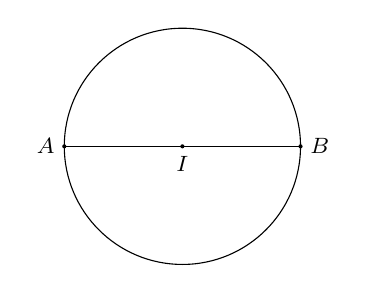
\begin{tikzpicture}[scale=.75,font=\footnotesize,line join=round,line cap=round,>=stealth]
				\draw  (0,0) circle (2cm);
				\fill (-2,0) circle  (1pt) node[left]{$A$};
				\fill (2,0) circle  (1pt) node[right]{$B$};
				\fill (0,0) circle (1pt) node[below]{$I$}; 
				\draw (-2,0)--(2,0); 
			\end{tikzpicture}
		} 
	} 
\end{bt}

% nguồn: MaHoaNH_TuLuan_Lop10
\begin{bt}%[0H9K3-2]%[ma:04cc6e48]
	Trong mặt  phẳng tọa độ $Oxy$.
	\begin{enumerate}
		\item Viết  phương trình đường tròn $(C)$ có tâm $I(-1;-2)$ và bán kính $R=\sqrt{10}$.
		\item Viết phương trình tiếp tuyến của đường tròn $(C)$, biết tiếp tuyến song song với đường thẳng  $(d)\colon x + 3y - 3=0$
	\end{enumerate}
	\loigiai{ 
		\begin{enumerate}
			\item  Ta có $(C)$ có tâm $I(-1;-2)$, $R=\sqrt{10}$ nên có phương trình là
			\allowdisplaybreaks 
			\begin{eqnarray*}
				(x-a)^2 +  (y-b)^2 = R^2 &\Leftrightarrow&
				(x+1)^2 + (y+2)^2 =  10.
			\end{eqnarray*}
			\item Gọi $(\Delta)$ là tiếp tuyến cần tìm.\\ 
			Vì $(\Delta)\parallel (d)\colon x + 3y -3 =0$ nên $(\Delta)\colon x  + 3y + m=0$ ($m\neq -3$).\\
			Vì $(\Delta)$  là tiếp tuyến của $(C)$ nên ta có
			\allowdisplaybreaks 
			\begin{eqnarray*}
				\mathrm{d}(I,\Delta)  = R
				&\Leftrightarrow& \dfrac{|1\cdot(-1) + 3\cdot (-2) + m |}{\sqrt{1^2 +  3^2}} =\sqrt{10}\\
				&\Leftrightarrow& \dfrac{|m-7|}{\sqrt{10}}=\sqrt{10}\\ 
				&\Leftrightarrow& |m-7|  = 10\\
				 &\Leftrightarrow& \hoac{&m-7 = 10\\& m-7 =-10.}\\
				 &\Leftrightarrow& \hoac{&m=17\quad (\text{nhận})\\&m=-3.\quad (\text{loại})}
			\end{eqnarray*}
			Vậy phương trình  tiếp tuyến cần tìm là $(\Delta)\colon x + 3y +17 =0$.
		\end{enumerate}
	} 
\end{bt}
